\section{Perceptron}
En 1943, Warren McCullock y Walter Pitts publican la primera aproximación de una
neurona simplificada, tratando de entender cómo funciona el cerebro biológico oara
el dieseño de inteligencia artificial, la llamada neurona McCullock-Pits (MCP)
\cite[see p10]{python}.

Las neuronas son células nerviosas interconectadas del cerebro que están involucradas
en el procesamiento y la transimición de señales químicas y eléctricas, como en la
siguiente figura:
\cite[e.g. page 300]{einstein}
\cite{einstein}

IMÁGEN

McCullock y Pitts describen a la neurona como una compuerta lógica sencilla con una
salida binaria; múltiples señales llegan a las dendritas para ser integradas al cuerpo
de la célula. Si la señal acumulada excede cierto umbral, se genera una señal de salida
que se le pasa al axón.

Unos años después, Frank Rosenblatt publica la primera aproximación al concepto de
perceptron basado en el modelo de neuronas MCP. FALTA REF. Intuitivamente, el algoritmo
aprende automáticamente los coeficientes de pesos óptimos que luego se multiplican
con las características de entrada para tomar la decisión de si la neurona se activa
o no. Este algoritmo podría ser usado entonces para predecir si una muestra pertenece
a una clase o a otra.

Formalmente, podemos plantearlo como un problema de clasificación binaria, donde nos
referimos a nuestras dos clases, por simplicidad, como 1 (clase positiva) y -1
(clase negativa). Definimos también una \textit{función de activación $\mathbf{\phi (z)}$}
que toma una combinación lineal de ciertos valores de entrada \textbf{x} y un
vector de pesos \textbf{w}, donde \textbf{z} es la llamada \textit{entrada de la red}
$(z = w_1x_1 + ... + w_mx_m)$:

\begin{equation*}
w=
    \begin{bmatrix}
        w_1 \\
        \vdots \\
        w_m
    \end{bmatrix}
    , x=
    \begin{bmatrix}
      x_1 \\
      \vdots \\
      x_m
    \end{bmatrix}
\end{equation*}
\\
Si la activación de una muestra particular $x^{(i)}$ es mayor que un parámetro definido
$\theta$, predecimos la clase 1, y la clase -1 en caso contrario. En el algoritmo
del perceptrón, la activación de función $\phi (\dot)$ es una \textit{función escalón},
que es llamada a veces la \textit{función de Heaviside}:
\begin{equation*}
  \phi(z)= \left\{ \begin{array} {rl}
    1 & \text{si } z \geq \theta \\
    -1 & \text{en otro caso} \end{array} \right.
\end{equation*}

Por simplicidad, definimios $w_0=-\theta$ y $x_0=1$, escribiendo entonces a $z$ de la
forma $z=w_0x_0 + w_1x_1 + \dots + w_mx_m = \mathbf{w^Tx}$.
La siguiente imágen ilustra cómo la entrada de la red $z=w^Tx$ es \textit{aplanada}
a una salida binaria (-1 o 1) por la función de activación del perceptrón (izquierda)
y cómo puede ser usada para discriminar entre dos clases linealmente separables (derecha):
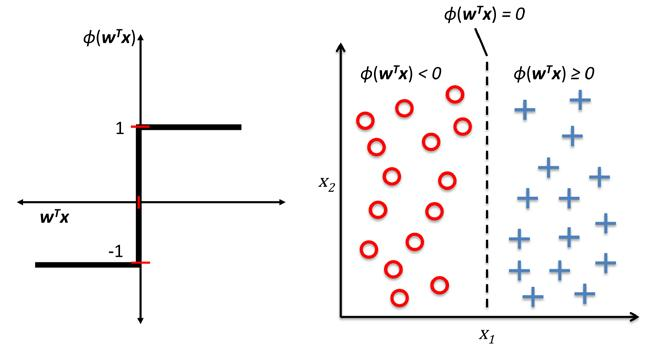
\includegraphics[scale=0.5]{perceptron}

La idea detrás del modelo de perceptron de Rosenblatt es reducir a una abstracción de cómo funciona
una neurona: se activa o no se activa. Así, la regla inicial de Roseblatt es relativamente
simple y puede ser resumida en los siguientes pasos:

1. Inicializar los pesos en cero o en números aleatorios cercanos a cero.

2. Para cada muestra de entrenamiento $x^{(i)}$ realizar los siguientes pasos:

1. Caluclar el valor de salida $\hat y$.
2. Actualizar los pesos.


En este caso, el valor de salida es la clasificación dada por la función escalón
definida previamente, y la actualización simultánea de cada peso $w_j$ en el
vector de pesos $w$ puede ser escrito más formalmente cómo:
\begin{equation}
  w_j := w_j + \Delta w_j
\end{equation}

El valor de $\Delta w_j$, que es usado para actualizar el peso $w_j$, es
calculado por la regla de aprendizaje de percetron:
\begin{equation}
  \Delta w_j = \eta (y^{(i)} - \hat y^{(i)})x^{(i)}_j
\end{equation}

Donde $\eta$ es el índice de aprendizaje (una constante entre 0 y 1),
$y^{(i)}$ es la clasificación real de la i-ésima muestra, y $\hat y^{(i)}$
es la clasificación dada por la predicción. Es importante resaltar que
todos los pesos en el vector de pesos son actualizados de manera
simultánea, lo que significa que no recalculamos $\hat y^{(i)}$ hasta que
todos los pesos $\Delta w_j$ han sido actualizados.

Podemos resumir el concepto general de perceptron con la siguiente imágen:
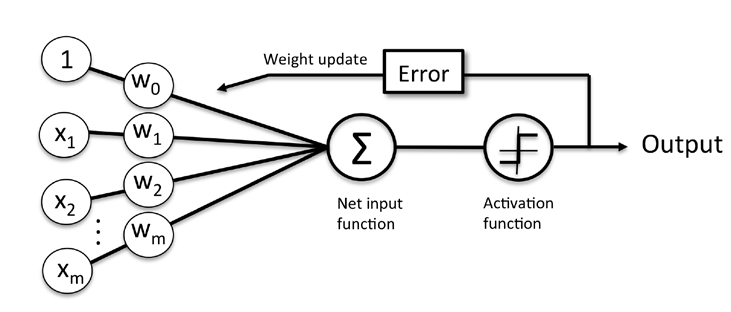
\includegraphics[scale=0.5]{perceptron-summary}

La imágen anterior muestra cómo el perceptron recibe las entradas de una
muestra $x$ y las combina con los pesos $w$ para calcular la entrada neta.
Esta entrada se le dá a la función de activación, que genera una salida
binaria (-1 o 1 en este caso), representando la predicción de la clasifica-
ción. Durante la fase de aprendizaje, la salida es usada para calcular el
error de la predicción y actualizar los pesos.
